% path to figures directory
\graphicspath{{img/chapter_5/}}

\chapter{The two-photon decay of a scalar-quirk bound state}
\label{chapter:quirk}

\begin{flushleft}
  \textit{This chapter is based on the publication `Explaining the
    \SI{750}{\GeV} diphoton excess with a coloured scalar charged under a new
    confining gauge interaction,' written in collaboration with Robert
    Foot~\cite{Foot:2016llc}. We use the extinct Greek letter $\digamma$ to
    represent a bound state of scalars charged under an unbroken
    $\mathrm{SU}(N)$, whose two-photon decay is posited to explain the
    \SI{750}{\GeV} diphoton excess, which similarly went extinct. The
    explanation in terms of the $\mathrm{SU}(N)$ bound state provides an
    especially simple explanation for the large production cross-section, which
    characterised the excess. Given the sensitivity of the diphoton channel to
    new physics, we hope that the conclusions of this paper still provide useful
    insight into how such a diphoton resonance might be explained economically.
    We note that this chapter is somewhat parenthetical to the earlier narrative
    of the thesis.}
\end{flushleft}

\section{Introduction}

An excess of events containing two photons with invariant mass near
\SI{750}{\GeV} has been observed in \SI{13}{\TeV} proton--proton collisions by
the ATLAS and CMS collaborations~\cite{ATLAS-CONF-2015-081, CMS:2015dxe}. The
cross section $\sigma(pp \rightarrow \gamma \gamma)$ is estimated to be
\begin{align}
  \begin{split}
    \sigma (p p \rightarrow \gamma \gamma) &=
    \begin{cases}
      (10 \pm 3)~\fb & \text{ATLAS} \\
      (6 \pm 3)~\fb & \text{CMS}
    \end{cases}
  \end{split}
\end{align}
and there is no evidence of any accompanying excess in the dilepton
channel~\cite{ATLAS-CONF-2015-070}. If we interpret this excess as the two
photon decay of a single new particle of mass $m$ then ATLAS data provide a hint
of a large width: $\Gamma/m \sim 0.06$, while CMS data prefer a narrow width.
Naturally, further data collected at the LHC should provide a clearer picture as
to the nature of this excess.

There has been vast interest in the possibility that the diphoton excess results
from physics beyond the SM. Most discussion has focused on models where the
excess is due to a new scalar particle which subsequently decays into two
photons \textit{e.g.} Ref.~\cite{Franceschini:2015kwy}. The possibility that the
new scalar particle is a bound state of exotic charged fermions has also been
considered, \textit{e.g.} Refs.~\cite{Kats:2016kuz, Curtin:2015jcv,
  Kamenik:2016izk, Ko:2016sht, Barrie:2016ndh}. Here we consider the case that
the \SI{750}{\GeV} state is a non-relativistic bound state constituted by an
exotic \textit{scalar} particle $\chi$ and its antiparticle, charged under
$\mathrm{SU}(3)_{c}$ as well as a new unbroken non-abelian gauge interaction.
Having $\chi$ be a scalar rather than a fermion is not merely a matter of taste:
in such a framework a fermionic $\chi$ would lead to the formation of bound
states which (typically) decay to two leptons more often than to photons; a
situation which is not favoured by the data.

The bound state, which we denote $\digamma$, can be produced through
gluon--gluon fusion directly (\textit{i.e.} at threshold
$\sqrt{s_{gg}} \simeq M_\digamma$) or indirectly via
$gg \rightarrow \chi^\dagger \chi \rightarrow \digamma + \textit{soft quanta}$
(\textit{i.e.} above $\digamma$ threshold: $\sqrt{s_{gg}} > M_\digamma$). The
indirect production mechanism can dominate the production of the bound state,
which is an interesting feature of this kind of theory.

\section{The model}

We take the new confining unbroken gauge interaction to be $\mathrm{SU}(N)$, and
assume that, like $\mathrm{SU}(3)_{c}$, it is asymptotically free and confining
at low energies. However, the new $\mathrm{SU}(N)$ dynamics is qualitatively
different from QCD as all the matter particles [assumed to be in the fundamental
representation of $\mathrm{SU}(N)$] are taken to be much heavier than the
confinement scale, $\Lambda_{N}$. In fact we here consider only one such matter
particle, $\chi$, so that $M_\chi \gg \Lambda_{N}$ is assumed. In this
circumstance a $\chi^\dagger \chi$ pair produced at the LHC above the threshold
$2M_\chi$ but below $4M_\chi$ cannot fragment into two jets. The
$\mathrm{SU}(N)$ string which connects them cannot break as there are no light
$\mathrm{SU}(N)$-charged states available. This is in contrast to heavy quark
production in QCD where light quarks can be produced out of the vacuum enabling
the colour string to break. The produced $\chi^\dagger\chi$ pair can be viewed
as a highly excited bound state, which de-excites by $\mathrm{SU}(N)$-ball and
soft glueball/pion emission~\cite{Carlson:1991zn}.

With the new unbroken gauge interaction assumed to be $\mathrm{SU}(N)$ the gauge
symmetry of the SM is extended to
\begin{equation}
  \label{eq:gaugegroup}
  \mathrm{SU(3)}_{c} \otimes \mathrm{SU}(2)_{L} \otimes \mathrm{U}(1)_{Y} \otimes \mathrm{SU}(N).
\end{equation}
This kind of theory can arise naturally in models which feature large colour
groups~\cite{Foot:1990jm, Foot:2011xu, Gherghetta:2016fhp} and in models with
leptonic colour~\cite{Foot:1990dw, Foot:1991fk, Foot:2006ie, Clarke:2011aa} but
was also considered earlier by Okun~\cite{Okun:1980mu}. The notation
\textit{quirks} for heavy particles charged under an unbroken gauge symmetry
(where $M_\chi \gg \Lambda_{N}$) was introduced in~\cite{Carlson:1991zn} where
the relevant phenomenology was examined in some detail in a particular
model\footnote{Some other aspects of such models have been discussed over the
  years, including the possibility that the $\mathrm{SU}(N)$ confining scale is
  low ($\sim$ \keV), a situation which leads to macroscopic
  strings~\cite{Kang:2008ea}.}. For convenience we borrow their nomenclature and
call the new quantum number \textit{hue} and the massless gauge bosons
\textit{huons} ($\mathcal{H}$).

The phenomenological signatures of the bound states (quirkonia) formed depend on
whether the quirk is a fermion or boson. Here we assume that the quirk $\chi$ is
a Lorentz scalar in light of previous work which indicated that bound states
formed from a fermionic $\chi$ state would be expected to be observed at the LHC
via decays of the spin-1 bound state into opposite-sign lepton pairs
($\ell^+\ell^-$)~\cite{Carlson:1991zn, Clarke:2011aa}. In fact, this appears to
be a serious difficulty in attempts to interpret the \SI{750}{\GeV} state as a
bound state of fermionic quirk particles (such as those of
Refs.~\cite{Kats:2016kuz, Curtin:2015jcv, Kamenik:2016izk}). The detailed
consideration of a scalar $\chi$ appears to have been largely
overlooked\footnote{The idea has been briefly mentioned in recent
  literature~\cite{Agrawal:2015dbf, Ko:2016sht}.}, perhaps due to the paucity of
known elementary scalar particles. With the recent discovery of a Higgs-like
scalar at \SI{125}{\GeV}~\cite{Aad:2012tfa, Chatrchyan:2012ufa} it is perhaps
worth examining signatures of scalar quirk particles. In fact, we point out here
that the two photon decay is the most important experimental signature of bound
states formed from electrically charged scalar quirks. Furthermore this
explanation is only weakly constrained by current data and thus appears to be a
simple and plausible option for the new physics suggested by the observed
diphoton excess.

\section{Explaining the excess}

The scalar $\chi$ that we introduce transforms under the extended gauge group
(Eq.~\ref{eq:gaugegroup}) as
\begin{equation}
  \chi \sim (\mathbf{3}, \mathbf{1}, Y; \mathbf{N}),
\end{equation}
where we use the normalisation $Q=Y/2$. The possibility that $\chi$ also
transforms non-trivially under $\mathrm{SU}(2)_{L}$ is interesting, however for
the purposes of this letter we focus on the $\mathrm{SU}(2)_{L}$ singlet case
for definiteness. Since two-photon decays of non-relativistic quirkonium will be
assumed to be responsible for the diphoton excess observed at the LHC, the mass
of $\chi$ will need to be around \SI{375}{\GeV}.

We have assumed that $\chi$ is charged under $\mathrm{SU}(3)_{c}$ so that it can
be produced at tree-level through QCD-driven pair production. We present the
production mechanisms in Fig.~\ref{fig:prod}. To estimate the production cross
section of the bound states, we first consider the indirect production mechanism
which we expect to be dominant. Here, a $\chi^\dagger \chi$ pair is produced
above threshold and de-excites emitting soft glueballs/pions and hueballs:
$gg \rightarrow \chi^\dagger \chi \rightarrow \digamma + \textit{soft quanta}$. We
first consider the case where the confinement scale of the new $\mathrm{SU}(N)$
interaction is similar to that of QCD. What happens in this case can be adapted
from the discussion in \cite{Carlson:1991zn}, where a fermionic quirk charged
under an unbroken $\mathrm{SU}(2)$ gauge interaction was considered. As already
briefly discussed in the introduction, the $\chi^\dagger \chi$ pairs initially
form a highly excited bound state, which subsequently de-excites in two stages.
The first stage is the non-perturbative regime where the hue string is longer
than $\Lambda_{N}^{-1}$. The second stage is characterised by a string scale
significantly less than $\Lambda_{N}^{-1}$: the perturbative Coulomb region.
Here the bound state can be characterised by the quantum numbers $n$ and $l$.
De-excitation continues until quirkonium is in a lowly excited state with
$l \leq 1$ and $n$. Imagine first that de-excitation continued until the ground
state ($n=1$, $l=0$) is reached. Given we are considering $\chi$ to be a scalar,
the quirkonium ground state, $\digamma$, will have spin 0, and is thus expected to
decay into SM gauge bosons and huons. The cross section
$\sigma(pp \rightarrow \digamma \rightarrow \gamma \gamma)$ in this case is then
\begin{equation}
  \sigma (pp \rightarrow \gamma \gamma) \approx \sigma(pp \rightarrow \chi^\dagger
  \chi) \times \text{Br}(\digamma \rightarrow \gamma \gamma).
\end{equation}
\begin{figure*}[t]
  \centering
  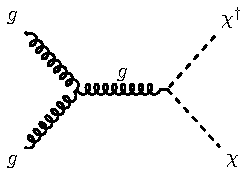
\includegraphics{d0.pdf}
  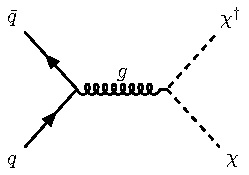
\includegraphics{d1.pdf}
  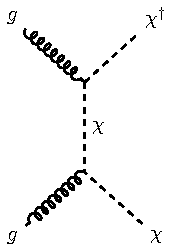
\includegraphics{d4.pdf}
  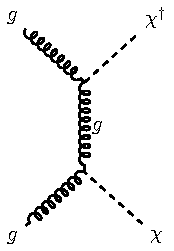
\includegraphics{d2.pdf}
  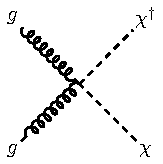
\includegraphics{d3.pdf}
  \caption{Tree-level pair production mechanisms for the scalar quirk $\chi$.}
  \label{fig:prod}
\end{figure*}

Since production is governed by QCD interactions, we can use the values of the
pair production cross sections for stops/sbottoms in the limit of decoupled
squarks and gluinos~\cite{Borschensky:2014cia}. For a $\chi$ mass of
\SI{375}{\GeV}
\begin{align}
  \begin{split} \label{eq:ind1}
    \sigma (p p \rightarrow \chi^\dagger \chi) &\approx
    \begin{cases}
      2.6 N \text{ pb} & \text{at \SI{13}{\TeV}} \\
      0.5 N \text{ pb} & \text{at \SI{8}{\TeV}}
    \end{cases} \ .
  \end{split}
\end{align}
The branching fraction is to leading order
\begin{equation}
  \text{Br}(\digamma \rightarrow \gamma \gamma) \simeq \frac{3NQ^4 \alpha^2}{\frac{2}{3}N \alpha_{s}^2
    + \frac{3}{2}C_{N}\alpha_{N}^2 + 3NQ^4\alpha^2},
  \label{eq:5a}
\end{equation}
where $C_{N} \equiv (N^2 - 1)/(2N)$, $\alpha_{N}$ is the new $\mathrm{SU}(N)$
interaction strength and we have neglected the small contribution of
$\digamma \rightarrow Z\gamma / ZZ$ to the total width. Eq.~\eqref{eq:5a} also
neglects the decay to Higgs particles: $\digamma \to hh$, which arises from the Higgs
potential portal term $\lambda_\chi \chi^\dagger \chi \phi^\dagger \phi$.
Theoretically this rate is unconstrained given the dependence on the unknown
parameter $\lambda_\chi$, but could potentially be important. However, limits
from resonant Higgs boson pair production derived from \SI{13}{\TeV} data:
$\sigma (pp \rightarrow X \rightarrow hh \rightarrow bbbb) \lesssim \SI{50}{\fb}$
at $M_X \approx \SI{750}{\GeV}$~\cite{ATLAS-CONF-2016-017, CMS-PAS-HIG-16-002}
imply that the Higgs decay channel must indeed be subdominant (\textit{c.f.}\
$\digamma \rightarrow gg$, $\mathcal{H}\mathcal{H}$).

The renormalised gauge coupling constants in Eq.~\eqref{eq:5a} are evaluated at
the renormalisation scale $\mu \sim M_\digamma/2$. Taking for instance the specific
case of $N=2$, $\alpha_{N} = \alpha_{s} \simeq 0.10$ (at
$\mu \sim M_\digamma/2$) gives
\begin{equation}
  \sigma (pp \rightarrow \gamma \gamma) \approx 5 \left( \frac{Q}{1/2} \right)^4~\fb \text{ at \SI{13}{\TeV}} \ .
\end{equation}
At $\sqrt{s} = \SI{8}{\TeV}$ the cross section is around five times smaller. We
present the cross section $\sigma(pp \rightarrow \digamma \rightarrow \gamma \gamma)$
for a range of masses $M_\digamma$ and different combinations of $Q$ and $N$ in
Fig.~\ref{fig:plot}. The parameter choice $\alpha_{N}=\alpha_{s}$ and
$\Lambda_{N}=\Lambda_{\text{QCD}}$ has been assumed. (The cross section is not highly
sensitive to $\Lambda_{N}$, $\alpha_{N}$ so long as we are in the perturbative
regime: $\Lambda_{N}\lesssim \Lambda_{\text{QCD}}$.) Evidently, for $N = 2$, a $\chi$
with electric charge $Q \approx 1/2$ is produced at approximately the right rate
to explain the diphoton excess.
\begin{figure*}[t]
  \begin{center}
    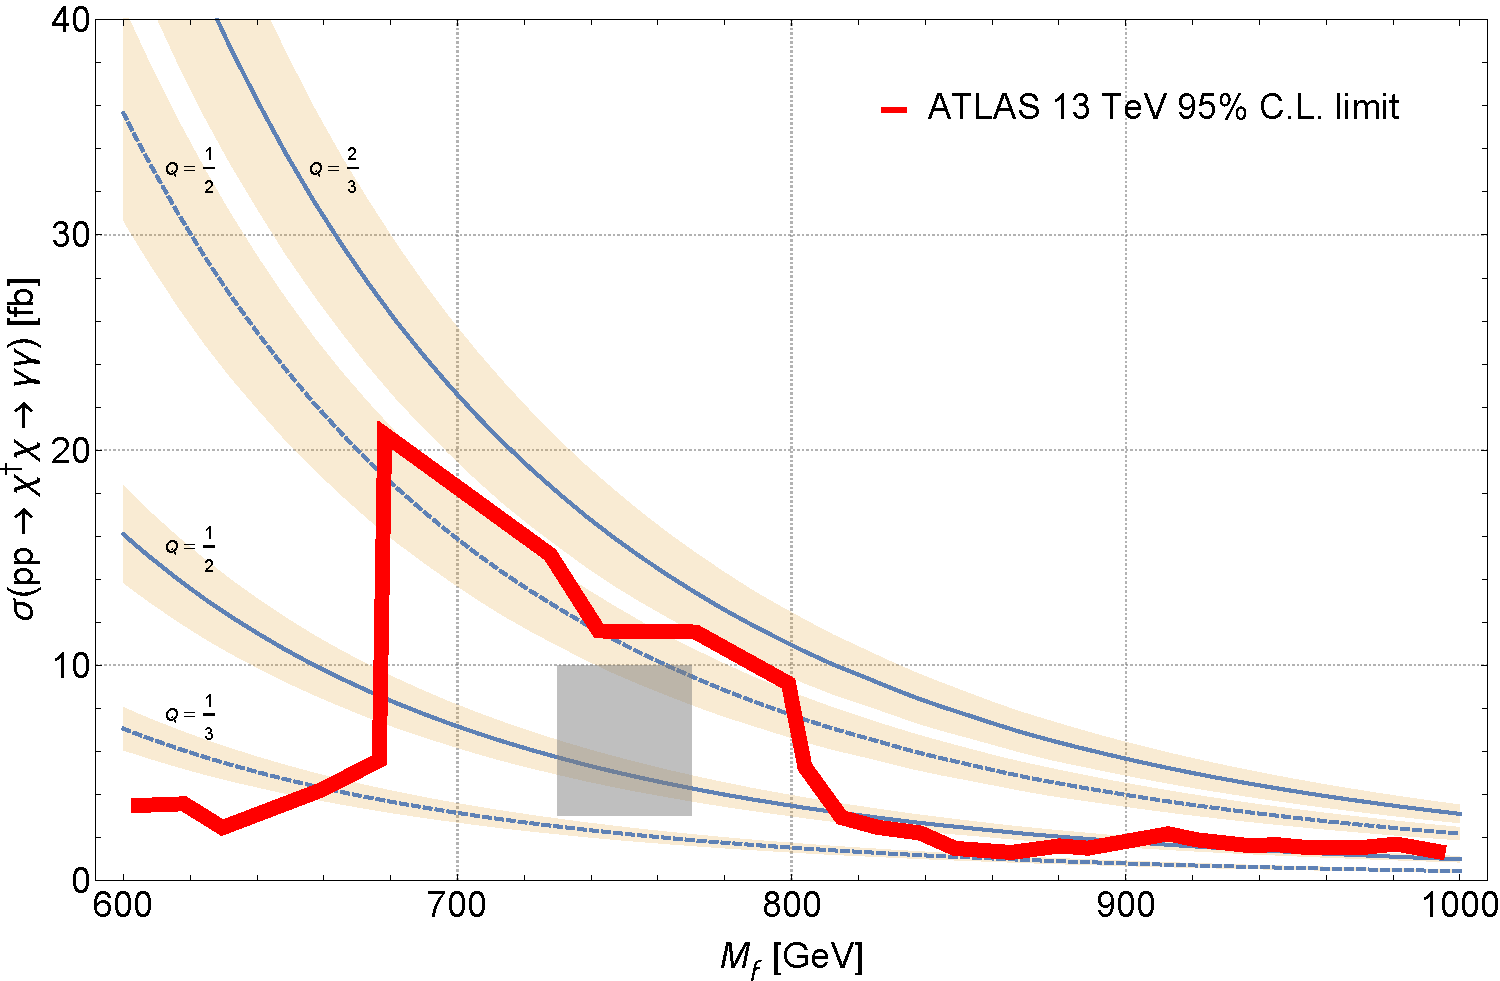
\includegraphics[scale=0.48]{plot.pdf}
    \caption[The cross section
    $\sigma(pp \rightarrow \digamma \rightarrow \gamma \gamma)$ at \SI{13}{\TeV} for
    a range of quirkonium masses $M_\digamma$ and charge assignments.]{The cross
      section $\sigma(pp \rightarrow \digamma \rightarrow \gamma \gamma)$ at
      \SI{13}{\TeV} for a range of quirkonium masses $M_\digamma$ and charge
      assignments. Solid lines denote choices of $N=2$ and dashed lines choices
      of $N=5$. The rectangle represents the $\sigma \in [3, 10]~\fb$ indicative
      region accommodated by the ATLAS and CMS data. The solid red line is the
      ATLAS \SI{13}{\TeV} exclusion limit. Uncertainties reflect error
      associated with the parton distribution functions.}
    \label{fig:plot}
  \end{center}
\end{figure*}

In practice de-excitation of the produced quirkonium does not always continue
until the ground state is reached. In this case annihilations of excited states
can also contribute. However those with $l=0$ will decay in the same way as the
ground state. The only difference is that the excited states will have a
slightly larger mass (which we will estimate in a moment) due to the change in
the binding energy. This detail could be important as it can effectively enlarge
the observed width. Annihilation of excited states with non-zero orbital angular
momentum could in principle also be important, however these are suppressed as
the radial wavefunction vanishes at the origin: $R(0) = 0$ for $l \geq 1$. They
are expected to de-excite predominately to $l=0$ states rather than
annihilate~\cite{Carlson:1991zn}. Nevertheless, for sufficiently large
$\alpha_{N}$ the $l=1$ annihilations: $\digamma \rightarrow \mu^+\mu^-$ and
$\digamma \rightarrow e^+e^-$ could potentially be observable.

The $l=0$ excited states can be characterised by the quantum number $n$ with
binding energies:
\begin{equation}
  \frac{E_n}{M_\digamma} = - \frac{1}{8n^2} \left[ \frac{4}{3} \bar{\alpha}_{s} + C_{N} \bar{\alpha}_{N} + Q^2 \bar{\alpha} \right]^2.
  \label{eq:8y}
\end{equation}
The above formula was adapted from known results with quarkonium, \textit{e.g.}\
\cite{Kats:2016kuz} (and of course also the hydrogen atom). The coupling
constants $\bar{\alpha}_{s}$, $\bar{\alpha}_{N}$ and $\bar{\alpha}$ are
evaluated at a renomalisation scale corresponding to the mean distance between
the particles which is of order the Bohr radius:
$a_0 = 4/[(4\bar{\alpha}_{s}/3 + C_{N}\bar{\alpha}_{N} + Q^2 \bar{\alpha})M_\digamma]$.
The bound state, described by the radial quantum number $n$ has mass given by
$M_\digamma(n) = 2M_\chi + E_n$. Considering as an example $N=2$ and
$\bar{\alpha}_{N} = \bar{\alpha}_{s} = 0.15$, $\bar{\alpha} = 1/137$ we find the
mass difference between the $n=1$ and $n=2$ states to be
$\Delta M = (E_1-E_2) \approx 0.01 M_\digamma$. Larger mass splittings will be
possible\footnote{Additional possibilities arise if $\chi$ transforms
  non-trivially under $\mathrm{SU}(2)_{L}$, \textit{i.e.}\ forming a
  representation $\mathbf{N}_{L}$. The mass degeneracy of the multiplet will be
  broken at tree-level by Higgs potential terms along with electroweak radiative
  corrections. The net effect is that the predicted width of the
  $pp \rightarrow \gamma \gamma$ bump can be effectively larger as there are
  $\mathrm{N}_{L}$ distinct bound states, $\digamma^i$, (of differing masses) which
  can each contribute to the decay width. Although each state is expected to
  have a narrow width, when smeared by the detector resolution the effect can
  potentially be a broad feature.} if $\bar{\alpha}_{N} > \bar{\alpha}_{s}$,
although it has been shown in the context of fermionic quirk models that the
phenomenology is substantially altered in this regime~\cite{Curtin:2015jcv}. In
particular, the hueballs can become so heavy that the decays of the bound state
into hueballs is kinematically forbidden.

In the above calculation of the bound state production cross section, we
considered only the \emph{indirect} production following pair production of
$\chi^\dagger \chi$ above threshold. The bound state can also be produced
directly: $gg \rightarrow \digamma$, where $\sqrt{s_{gg}} \approx M_\digamma$. The cross
section of the ground state direct resonance production is
\begin{equation}
  \sigma (pp \rightarrow \digamma)_{\text{DR}} \approx \frac{C_{gg} K_{gg} \Gamma (\digamma \rightarrow gg)}{s M_\digamma},
\end{equation}
where $C_{gg}$ is the appropriate parton luminosity coefficient and $K_{gg}$ is
the gluon NLO QCD K-factor. For $\sqrt{s} = \SI{13}{\TeV}$ we take
$C_{gg} \approx 2137$~\cite{Franceschini:2015kwy} and
$K_{gg} = 1.6$~\cite{Harlander:2005rq}. The partial width
$\Gamma (\digamma \rightarrow gg)$ of the $n=1$, $l=0$ ground state is given by
\begin{equation}
  \Gamma (\digamma \rightarrow gg) =  \frac{4}{3} M_\digamma N \alpha_{s}^2
  \frac{|R(0)|^2}{M_\digamma^3} ,
\end{equation}
where the radial wavefunction at the origin for the ground state is:
\begin{equation}
  \frac{|R(0)|^2}{M_\digamma^3} = \frac{1}{16} \left[
    \frac{4}{3} \bar \alpha_s + C_{N} \bar{\alpha}_{N} + Q^2 \bar{\alpha}
  \right]^3.
  \label{eq:11y}
\end{equation}
Considering again the example of $N=2$ and
$\bar{\alpha}_{N} = \bar{\alpha}_{s} = 0.15$, $\bar{\alpha} = 1/137$ we find
\begin{equation}
  \sigma(pp \rightarrow \digamma)_{DR} \approx \SI{0.40}{\pb} \quad \text{at \SI{13}{\TeV}} \ .
\end{equation}
Evidently, the direct resonance production cross section is indeed expected to
be subdominant, around 8\% that of the indirect production cross section
(Eq.~\ref{eq:ind1})\footnote{If $\bar{\alpha}_{N}$ is sufficiently large, one
  can potentially have direct resonance production comparable or even dominating
  indirect production (such a scenario has been contemplated recently in
  \cite{Kamenik:2016izk, Ko:2016sht}). Naturally at such large
  $\bar{\alpha}_{N}$ the perturbative calculations become unreliable, and one
  would have to resort to non-perturbative techniques such as lattice
  computations.}.

We now comment on the regime where $\Lambda_{N}$ is smaller than
$\Lambda_{\text{QCD}}$. In fact, if the $\mathrm{SU}(N)$ confining scale is only
a little smaller than $\Lambda_{\text{QCD}}$ then a light quark pair can form
out of the vacuum, leading to a bound state of two QCD colour singlet states:
$\chi \bar{q}$ and $\chi^\dagger q$. These colour singlet states would
themselves be bound together by $\mathrm{SU}(N)$ gauge interactions to form the
$\mathrm{SU}(N)$ singlet bound state. Since only $\mathrm{SU}(N)$ interactions
bind the two composite states ($\chi \bar{q}$ and $\chi^\dagger q$), it follows
that
$\frac{4}{3} \bar \alpha_s + C_{N} \bar{\alpha}_{N} + Q^2 \bar{\alpha} \to C_{N} \bar{\alpha}_{N} + (Q - Q_q)^2 \bar{\alpha}$
in Eqs.~\ref{eq:8y} and \ref{eq:11y}. Therefore if the confinement scale of
$\mathrm{SU}(N)$ is smaller than that of QCD then the direct production rate
becomes completely negligible relative to the indirect production mechanism. The
rate of $\digamma$ production is the same as that found earlier in
Eq.~\ref{eq:ind1}, but the branching ratio to two photons is modified:
\begin{equation}
  \text{Br}(\digamma \rightarrow \gamma \gamma) \simeq \frac{3NQ^4 \alpha^2}{\frac{7}{3}N\alpha_{s}^2
    + \frac{3}{2} C_{N} \alpha_{N}^2 + 3NQ^4\alpha^2},
\end{equation}
where, as before, we have neglected the small contribution of $\digamma \rightarrow
Z\gamma / ZZ$ to the total width, and also the contribution from $\digamma \rightarrow hh$.
In this regime somewhat larger values of $Q$ can be accommodated, such as $Q = 5/6$ for $N=2$ \footnote{
  Although it is perhaps too early to speculate on the possible role of $\chi$ in a more elaborate framework,
  we nevertheless remark here that particles fitting its description are required for spontaneous symmetry breaking of
  extended Pati--Salam type unified theories~\cite{Foot:1990ij}.}.


Notice that in the $\Lambda_{N} < \Lambda_{\text{QCD}}$ regime the
size of the mass splittings between the excited states becomes small as
$\frac{4}{3} \bar \alpha_s + C_{N} \bar{\alpha}_{N} + Q^2 \bar{\alpha} \to
C_{N} \bar{\alpha}_{N} + (Q - Q_q)^2 \bar{\alpha} $ in Eq.~\ref{eq:8y}. We therefore
expect no effective width enhancement due to the excited state decays at the LHC
in the small $\Lambda_{N}$ regime. Of course a larger effective width is still possible if there are
several nearly degenerate scalar quirk states, which, as briefly mentioned earlier,
can arise if $\chi$ transforms nontrivially under $\mathrm{SU}(2)_{L}$.


\section*{Other signatures}

While the two photon decay channel of the bound state should be the most
important signature, the dominant decay is expected to be via $\digamma \rightarrow
gg$ and $\digamma \rightarrow \mathcal{H} \mathcal{H}$. The former process is
expected to lead to dijet production while the latter will be an invisible
decay. The dijet cross section is easily estimated:
\begin{align}
  \begin{split}
    \sigma (p p \rightarrow jj) &\approx
    \begin{cases}
      2.6 N \times \text{Br}(\digamma \rightarrow gg) \text{ pb} & \text{at \SI{13}{\TeV}} \\
      0.5 N \times \text{Br}(\digamma \rightarrow gg) \text{ pb} & \text{at \SI{8}{\TeV}}
    \end{cases}.
  \end{split}
\end{align}
The limit from \SI{8}{\TeV} data is $\sigma(pp \rightarrow jj) \lesssim 2.5$
pb~\cite{Aad:2014aqa, Khachatryan:2015dcf}. If gluons dominate the $\digamma$ decays
(i.e. $\text{Br}(\digamma \rightarrow gg) \approx 1$) then this experimental limit is
satisfied for $N \leq 5$. For sufficiently large $\alpha_{N}$ the invisible
decay can be enhanced, thereby reducing $\text{Br}(\digamma \rightarrow gg)$. In this
circumstance the bound on $N$ from dijet searches would weaken.

The invisible decays $\digamma \rightarrow \mathcal{H} \mathcal{H}$ are not expected
to lead to an observable signal at leading order for much of the parameter space
of interest\footnote{Scalar quirk loops can mediate hueball decays into gluons
  and other SM bosons~\cite{Carlson:1991zn, Juknevich:2009ji, Juknevich:2009gg}. The decay
  rate is uncertain, depending on the non-perturbative hueball dynamics.
  However, if the hueballs are able to decay within the detector then they can
  lead to observable signatures including displaced vertices. This represents
  another possible collider signature of the model.}. However, the
bremsstrahlung of a hard gluon from the initial state:
$pp \rightarrow \digamma g \rightarrow \mathcal{H}\mathcal{H} g$ can lead to a jet
plus missing transverse energy signature. Current data are not expected to give
stringent limits from such decay channels, however this signature could become
important when a larger data sample is collected. Note though that the rate will
become negligible in the limit that $\alpha_{N}$ becomes small. Also, in the
small $\Lambda_{N}$ regime, where the bound state is formed from $\chi \bar{q}$
and $\chi^\dagger q$, the two-body decay $\digamma \rightarrow g \gamma$
($\text{jet} + \text{photon}$) will also arise as in this case the scalar quirk
pair is not necessarily in the colour singlet configuration. The decay rate at
leading order is substantial:
\begin{equation}
  \frac{\Gamma(\digamma \rightarrow j\gamma)}{\Gamma(\digamma \rightarrow \gamma \gamma)} = \frac{8\alpha_s}{3\alpha Q^2}\ .
\end{equation}
Nevertheless, we estimate that this is still consistent with current data
\cite{Aad:2015ywd}, but would be expected to become important when a larger data
sample is collected.

Another important signature of the model will be the $pp \rightarrow \digamma \rightarrow Z\gamma$
and $pp \rightarrow \digamma \rightarrow ZZ$ processes. The rates of these decays, relative to $\digamma
\rightarrow \gamma \gamma$, are estimated to be:
\begin{align}
  \begin{split}
    \frac{\Gamma (\digamma \rightarrow Z \gamma) }{\Gamma (\digamma \rightarrow \gamma \gamma)} &= 2 \tan^2 \theta_{W},\\
    \frac{\Gamma (\digamma \rightarrow Z Z) }{\Gamma (\digamma \rightarrow \gamma \gamma)} &= \tan^4 \theta_{W}.
  \end{split}
\end{align}
If $\chi$ transforms non-trivially under $\mathrm{SU}(2)_{L}$ then deviations
from these predicted rates arise along with the tree-level decay
$\digamma \rightarrow W^+ W^-$.

\section{Conclusions}

We have considered a charged scalar particle $\chi$ of mass around
\SI{375}{\GeV} charged under both $\mathrm{SU}(3)_{c}$ and a new confining gauge
interaction (assigned to be $\mathrm{SU}(N)$ for definiteness). These
interactions confine $\chi^\dagger\chi$ into non-relativistic bound states whose
decays into photons can explain the \SI{750}{\GeV} diphoton excess observed at
the LHC. Taking the new confining group to be $\mathrm{SU}(2)$, we found that
the diphoton excess required $\chi$ to have electric charge approximately
$Q \sim [\frac{1}{2}, 1]$. An important feature of our model is that the exotic
particle $\chi$ has a mass much greater than the $\mathrm{SU}(N)$-confinement
scale $\Lambda_{N}$. In the absence of light $\mathrm{SU}(N)$-charged matter
fields this makes the dynamics of this new interaction qualitatively different
to that of QCD: pair production of the scalars and the subsequent formation of
the bound state dominates over direct bound state resonance production (at least
in the perturbative regime where $\Lambda_{N} \lesssim \Lambda_{\text{QCD}}$).
Since $\chi$ is a Lorentz scalar, decays of $\chi^\dagger \chi$ bound states to
lepton pairs are naturally suppressed, and thus constraints from dilepton
searches at the LHC can be ameliorated. This explanation is quite weakly
constrained by current searches and data from the forthcoming run at the LHC
will be able to probe our scenario more fully. In particular, dijet, mono-jet,
di-Higgs and $\text{jet} + \text{photon}$ searches may be the most promising
discovery channels.
